\section{浅层神经网络}
\subsection{浅层神经网络前向计算}
浅层神经网络的前向计算如图\ref{fig:forward_calc}所示。
\begin{figure}[htb]			% figure 浮动图片,htb选项用的最多
	\centering
	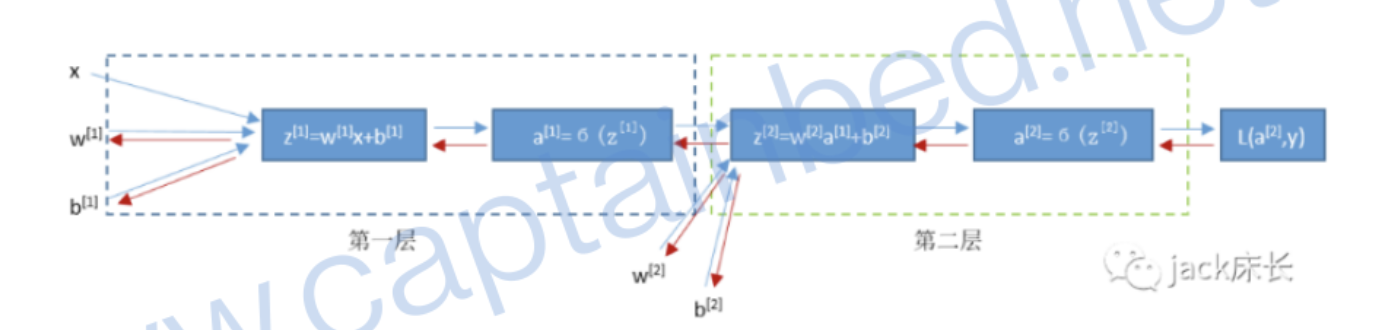
\includegraphics[width=8cm, height=3cm]{pictures/浅层神经网络/forward_calc}
	\caption{前向计算图}
	\label{fig:forward_calc}
\end{figure}

\subsection{深度神经网络训练的计算过程}
\textbf{任何一个神经网络的训练,大致可以划分为4个过程:}
循环迭代
\textbf{1.前向传播}
x, w, b => $y', caches$
其中y'是计算出来的结果,caches存放的是每一层的w,b,a,即caches = [(w1,b1,a1), (w2,b2,a2)...],其中a1就是x,缓存中间数据caches的目的是为了计算方向传播的梯度
举例,z=wa+b:
dz/dw = a
dz/db = 1
dz/da = w